\documentclass{article}
\usepackage{spalign}
\usepackage{graphicx}
\usepackage{amsmath}
\usepackage{amsfonts}
\usepackage{xcolor}

\title{Module 1 \textendash{} Linear Systems and Span \\
        Topic 1 \textendash{} Systems of Linear Equations \\
        Lesson 1 \textendash{} Solution Sets of Linear Equations}
\author{John Guzauckas}
\date{05/16/2022}

\begin{document}
\maketitle

\section{Topics}
We will explore the following concepts:

\begin{itemize}
    \item Systems of Linear Equations
    \item Elementary Row Operations
\end{itemize}

\section{Learning Objectives:}
Students should be able to do the following after watching the video and
completing the assigned homework:

\begin{itemize}
    \item Apply elementary row operations to solve systems of linear equations.
\end{itemize}

\section{A Single Linear Equation}
A linear equation has the form
\[a_{1}x_{1} + a_{2}x_{2} + \cdots + a_{n}x_{n} = b\]
$a_{1}$, $a_{2}$, $\dots$, $a_{n}$ and $b$ are the \textbf{coefficients}, 
$x_{1}$, $x_{2}$, $\dots$, and $x_{n}$ are the \textbf{variables}, 
and $n$ is the \textbf{dimension}, or number of variables.\\
For example:

\begin{itemize}
    \item $2x_{1} + 4x_{2} = 4$ is a line in 2 dimensions
    \item $3x_{1} + 2x_{2} + x_{3} = 6$ is a plane in 3 dimensions
\end{itemize}

\section{Systems of Linear Equations}
When we have one or more linear equations, we have a
\textbf{Linear System} of equations.\\
For example, a linear system with two equations is
\spalignsysdelims..
\[
  \spalignsys{
    x_{1} + 1.5x_{2} + \pi x_{3} = 4;
    5x_{1} \+ \. + 7x_{3} = 5
  }
\]
The set of all possible values of $x_{1}$, $x_{2}$, $\dots$, $x_{n}$
that satisfy all equations is the \textbf{solution set}. One point
in the solution set is a \textbf{solution}.

\section{Two Variable Case}
Consider the following systems. How are they different from each other?
\[
\begin{array}{ c c c }
    \spalignsys{x_{1} - 2x_{2} = -1;-x_{1} + 3x_{2} = 3} &
    \spalignsys{x_{1} - 2x_{2} = -1;-x_{1} + 2x_{2} = 1} &
    \spalignsys{x_{1} - 2x_{2} = -1;-x_{1} + 2x_{2} = 3} \\
    \\
    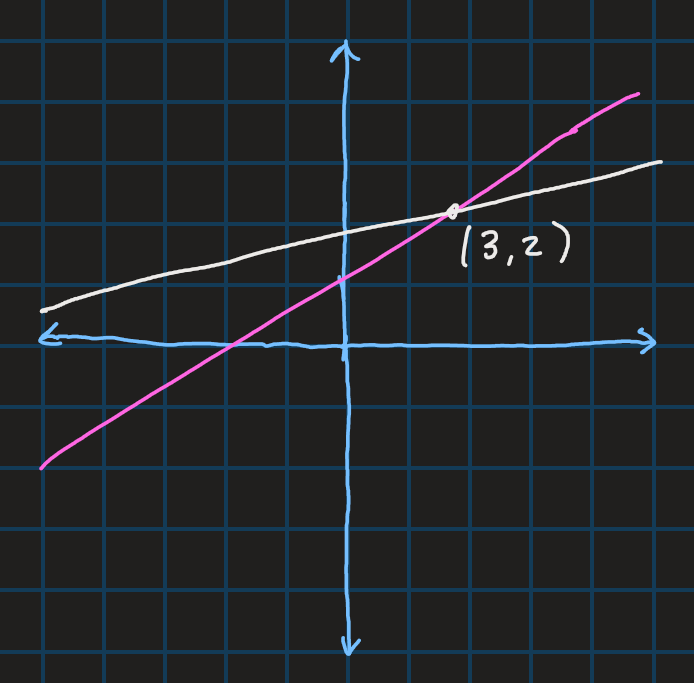
\includegraphics[scale=0.17]{Images/1.1.graph1.png} &
    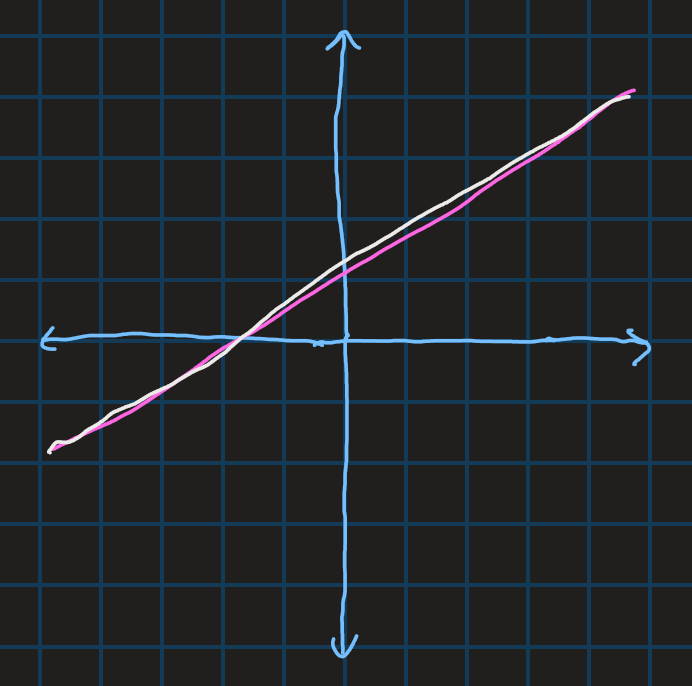
\includegraphics[scale=0.17]{Images/1.1.graph2.png} &
    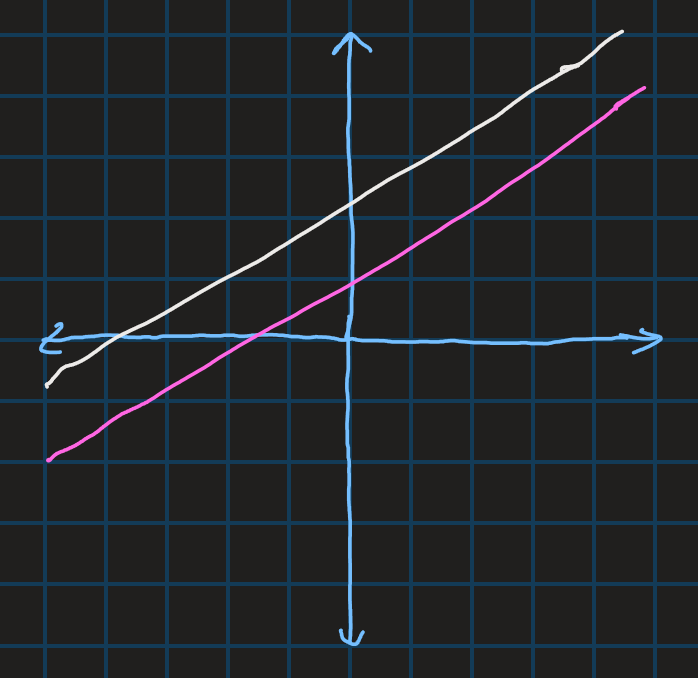
\includegraphics[scale=0.17]{Images/1.1.graph3.png} \\
    \text{Non-Parallel Lines} &
    \text{Identical Lines} &
    \text{Parallel Lines} \\
    \text{Unique Solution} &
    \text{Infinite Solutions} &
    \text{No Solutions} \\
\end{array}
\]

\section{Three Variable Case}
An equation $a_{1}x_{1} + a_{2}x_{2} + a_{3}x_{3} = b$ defines a plane
in $\mathbb{R}$. The \textbf{solution} to a system of \textbf{three equations}
is the set of points where all three planes intersect:

\begin{tabular}{ c c c }
    \\
    Planes Intersect At a Point &
    Planes Intersect On a Line &
    Parallel Planes \\
    \\
    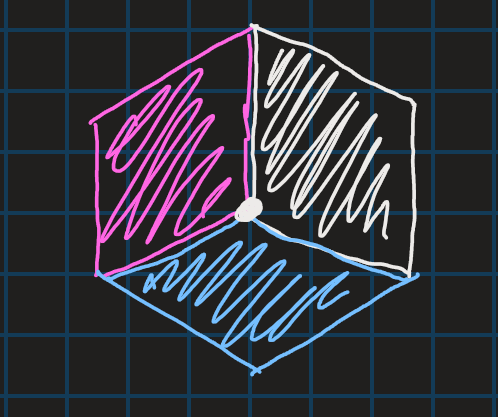
\includegraphics[scale=0.25]{Images/1.1.graph4.png} &
    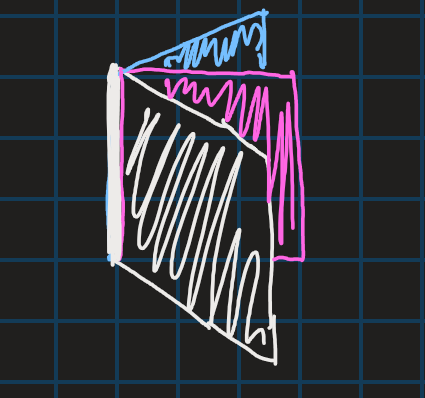
\includegraphics[scale=0.25]{Images/1.1.graph5.png} &
    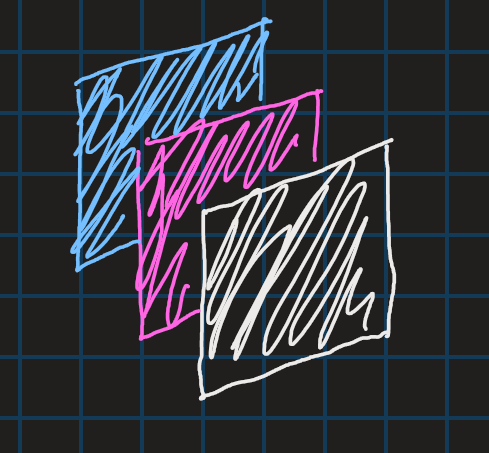
\includegraphics[scale=0.25]{Images/1.1.graph6.png} \\
    \\
    Unique Solution &
    Infinite Solutions &
    No Solutions \\
\end{tabular}

\section{Row Reduction by Elementary Row Operations}
How can we find the solution set to a set of linear equations?
\\
We can manipulate equations in a linear system using \textbf{row operations}:
\begin{enumerate}
    \item (Replacement/Addition) Add a multiple of one row to another
    \item (Interchange) Interchange/swap two rows
    \item (Scaling) Multiple a row by a non-zero scalar
\end{enumerate}
Let's use these operations to solve a system of equations:

\[
  \spalignsys{
    {\color{blue}R_{1}} \+ x_{1} - 2x_{2} + x_{3} = 0;
    {\color{blue}R_{2}} \+ \. \+ 2x_{2} - 8x_{3} = 8;
    {\color{blue}R_{3}} \+ 5x_{1} \+ \. - 5x_{3} = 10;
    ;
    {\color{blue}R_{1} + R_{2} \rightarrow R_{1}} \+ x_{1} + 0x_{2} - 7x_{3} = 8;
    {\color{blue}\frac{1}{2} \times R_{2} \rightarrow R_{2}} \+ \. \+ x_{2} - 4x_{3} = 4;
    {\color{blue}R_{3} - 5 \times R_{1} \rightarrow R_{3}} \+ \. \+ 10x_{2} - 10x_{3} = 10;
    ;
    {\color{blue}R_{1}} \+ x_{1} \+ \. - 7x_{3} = 8;
    {\color{blue}R_{2}} \+ \. \+ x_{2} - 4x_{3} = 4;
    {\color{blue}R_{3} - 10 \times R_{2} \rightarrow R_{3}} \+ \. \+ \. \+ 30x_{3} = -30;
    ;
    }
\]
Solve {\color{blue}$R_{3}$} $\Longrightarrow 30x_{3} = -30 \Longrightarrow x_{3} = -1$
\\
Substitute $x_{3} = -1$ into {\color{blue}$R_{1}$} $\Longrightarrow x_{1} - 7(-1) = 8
    \Longrightarrow x_{1} + 7 = 8 \Longrightarrow x_{1} = 1$
\\
Substitute $x_{3} = -1$ into {\color{blue}$R_{2}$} $\Longrightarrow x_{2} - 4(-1) = 4
    \Longrightarrow x_{2} + 4 = 4 \Longrightarrow x_{2} = 0$
\\
Our solution is the point $(1, 0, -1)$

\section{Summary}
We explored the following concepts in this video:
\begin{itemize}
    \item Systems of linear equations
    \item Elementary row operations
    \item Applying elementary row operations to solve a linear system
\end{itemize}

\section{Practice 1}
Consider the following linear system:

\[
  \spalignsys{
    {\color{blue}R_{1}} \+ x_{1} + x_{2} \+ \. = 1;
    {\color{blue}R_{2}} \+ \. \+ x_{2} + x_{3} = 3;
    {\color{blue}R_{3}} \+ \. \+ \. \+ x_{3} = 1;
    }
\]
\\
Substitute $x_{3} = 1$ into {\color{blue}$R_{2}$} $\Longrightarrow x_{2} + 1 = 3
    \Longrightarrow x_{2} = 2$
\\
Substitute $x_{2} = 2$ into {\color{blue}$R_{1}$} $\Longrightarrow x_{1} + 2 = 1
    \Longrightarrow x_{1} = -1$
\\
The solution is the point $(-1, 2, 1)$

\section{Practice 2}
Consider the linear system below:

\[
    \spalignsys{
        {\color{blue}R_{1}} \+ x + 2y = 4;
        {\color{blue}R_{1}} \+ c_{1}x + 6y = 1
    }\]
\\
The coefficient $c_{1}$ is a real number. For what value of $c_{1}$ are there
no solutions to this linear system?
\\
\\
No solution means that the one equation is a scalar multiple of the other, so
$k(x + 2y) = c_{1}x + 6y$
\\
$\Longrightarrow kx + 2ky = c_{1}x + 6y \Longrightarrow kx = c_{1}x$ and $2ky = 6y$
\\
$\Longrightarrow k = c_{1}$ and $2k = 6 \Longrightarrow k = c_{1}$ and $k = 3$
\\
So $c_{1} = 3$ causes the linear system to have no solutions.

\end{document}